%%%%%%%%%%%%%%%%%%%%%%%%%%%%%%%%%%%%%%%%%%%%%%%%%%%%%%%%%%%%%%%%%%%%%%%%%%%%%%%%%%
\begin{frame}[fragile]\frametitle{}
\begin{center}
{\Large Introduction to Probability}
\end{center}
\end{frame}

%%%%%%%%%%%%%%%%%%%%%%%%%%%%%%%%%%%%%%%%%%%%%%%%%%%%%%%%%%
\begin{frame}{Why Probability?}
\begin{itemize}
\item Real life scenarios are inherently random or too complex to be completely known. 
\item If you knew every ``Physics'' aspect of motion of a dice, you could predict the outcome, deterministically.
\item However this can never be done in practice, so there is a CHANCE of something happening.
\end{itemize}
\end{frame}

%%%%%%%%%%%%%%%%%%%%%%%%%%%%%%%%%%%%%%%%%%%%%%%%%%%%%%%%%%
\begin{frame}{Probability: the Likeliness}
\begin{itemize}
\item How likely something is to happen. 
\item Many events can't be predicted with total certainty. 
\item The best we can say is how likely they are to happen, using the idea of probability. 
\item Probability is the fraction of time that outcome would occur with repeated experiments.
\end{itemize}
\end{frame}

%%%%%%%%%%%%%%%%%%%%%%%%%%%%%%%%%%%%%%%%%%%%%%%%%%%%%%%%%%
\begin{frame}{Probability: Example}
\begin{itemize}
\item Probability (event ) = Number of ways it can happen / Total number of 
outcomes 
\item Example: the chances of rolling a ``4'' with a die 
\item Number of ways it can happen: 1 (there is only 1 face with a ``4'' on it) 
\item Total number of outcomes: 6 (there are 6 faces altogether) 
 \item Probability of  this event  = 1/ 6 
\end{itemize}
\end{frame}

%%%%%%%%%%%%%%%%%%%%%%%%%%%%%%%%%%%%%%%%%%%%%%%%%%%%%%%%%%
\begin{frame}{Probability: Example}
\begin{itemize}
\item There are 5 marbles in a bag: 4 are blue, and 1 is red. 
\item What is the probability that a blue marble gets picked? 
\item Number of ways it can happen: 4 (there are 4 blues) 
\item Total number of outcomes: 5 (there are 5 marbles in total) 
 
\item Probability of  this event  = 4 / 5 
\end{itemize}
\end{frame}

%%%%%%%%%%%%%%%%%%%%%%%%%%%%%%%%%%%%%%%%%%%%%%%%%%%%%%%%%%
\begin{frame}{Probability: Example}
\begin{itemize}
\item Flip 3 coins. What is the probability that we get exactly two heads?
\item Flip 1 coin, you get either H or T. Then flip 2nd coin, draw further branches (like below)
\item At the end you will have 8 possible outcomes
\begin{center}
\includegraphics[width=0.5\linewidth,keepaspectratio]{math1}
\end{center}

\tiny{(Ref: Math for Machine Learning - AWS Brent Werness)}

\item What we want are HHT, HTH, THH. So 3 out of 8. 
\item Probability of  this event  = 3 / 8

\end{itemize}


\end{frame}


%%%%%%%%%%%%%%%%%%%%%%%%%%%%%%%%%%%%%%%%%%%%%%%%%%%%%%%%%%
\begin{frame}{Probability} 
\begin{definition}
Given an experiment, let $S$ be the set of all possible outcomes ($S$ is often called the \underline{sample space}) and $A$ be the event of some particular outcomes (so $A\subseteq S$).  The probability of $A$, denoted by $P(A)$, is the relative proportion of $A$ in $S$.
\end{definition}

\end{frame}

%%%%%%%%%%%%%%%%%%%%%%%%%%%%%%%%%%%%%%%%%%%%%%%%%%%%%%%%%%
\begin{frame}{Probability} 
\begin{example}
Suppose we are rolling a fair die, then $S=\{1,2,3,4,5,6\}$.  Let $A$ be the event that the outcome is an even number, that is, $A=\{2,4,6\}$.  Then $P(A)= 1/2$.
\end{example}

\begin{example}
Suppose we are rolling two fair dice, and let $A$ be the event that the sum of outcomes is either 6 or 7.  Then $P(A)= 11/35$.
\end{example}
\end{frame}

%%%%%%%%%%%%%%%%%%%%%%%%%%%%%%%%%%%%%%%%%%%%%%%%%%%%%%%%%%
\begin{frame}{Some terminologies }
\begin{itemize}
\item Experiment or Trial: an action where the result is uncertain. Example: Tossing a coin, throwing dice are examples of experiments. 
\item Outcome: A single possibility from the experiment. E.g. $\Omega = {HHT, THT, \ldots}$, each of these are outcomes.
\end{itemize}
\end{frame}

%%%%%%%%%%%%%%%%%%%%%%%%%%%%%%%%%%%%%%%%%%%%%%%%%%%%%%%%%%
\begin{frame}{Event}
\begin{itemize}
\item Event: a set of outcomes/results of an experiment 
 \item An event is what we are looking for ue $E={ExactlyTwoHeads}$. E is any subset of the sample space. The set of all events associated with a given
experiment is called the event space.
\item Example Events: 
\begin{itemize}
\item Getting a Tail when tossing a coin is an event 

\item Rolling a ''5'' is an event. 
\end{itemize}
\item An event can include one or more possible outcomes: 
\begin{itemize}
\item Choosing a ''King'' from a deck of cards (any of the 4 Kings) is an 
event 
\item Rolling an ''even number'' (2, 4 or 6) is also an event 
\end{itemize}
\end{itemize}
\end{frame}

%%%%%%%%%%%%%%%%%%%%%%%%%%%%%%%%%%%%%%%%%%%%%%%%%%%%%%%%%%
\begin{frame}
\frametitle{Sample space }
\begin{itemize}
\item  
Sample Space: all the possible outcomes of an experiment. Example: choosing a card from a deck 
\begin{itemize}
\item There are 52 cards in a deck (not including Jokers) 
\item So  the  Sample  Space  is  all  52  possible  cards:  {Ace  of  Hearts,  2  of 
Hearts, etc. } 
\end{itemize}
\item A Sample Point is just one possible outcome. 
\item And an Event can be one or more of the possible outcomes. 
\item Flipping the coin:  the sample space is  $\{H,T\}$.

\item Whats the sample space of number of heads if we flip a coin 10 times?

\item $\{0,1,\ldots,10\}$

\end{itemize}
\end{frame}

%%%%%%%%%%%%%%%%%%%%%%%%%%%%%%%%%%%%%%%%%%%%%%%%%%%%%%%%%%
\begin{frame}
\frametitle{Probability of an event? }
\begin{itemize}
\item  Both `event' and `probability' are intuitively understood by most 
people, but we need to establish certain rules. 
\item  `Rain tomorrow', `3 or fewer cyclones next year', `Crop yield will 
exceed a given threshold' are  all examples of `events' whose 
`probabilities' might be of interest. 
\end{itemize}

\begin{center}
\includegraphics[width=0.65\linewidth,keepaspectratio]{evsamp}
\end{center}
\end{frame}


%%%%%%%%%%%%%%%%%%%%%%%%%%%%%%%%%%%%%%%%%%%%%%%%%%%%%%%%%%%
\begin{frame}
\frametitle{Event probabilities}

An {\bf event} is a set of one or more points in the sample space.
The probability of an event is the sum of the probabilities for the
points in the event.

\textcolor{blue}{\bf Example:} Consider this distribution:

\begin{center}
\begin{tabular}{ll}
{$x$} & {$P(X=x)$}\\\hline 
Favorable & \hspace{0.8cm}0.3 \\
Neutral & \hspace{0.8cm}0.5 \\
Unfavorable & \hspace{0.8cm}0.2 \\\hline
\end{tabular}
\end{center}

The response being either \textcolor{purple}{favorable or neutral} is
an event, and this event has probability $0.3+0.5=0.8$.

\end{frame}

%%%%%%%%%%%%%%%%%%%%%%%%%%%%%%%%%%%%%%%%%%%%%%%%%%%%%%%%%%%
\begin{frame}
\frametitle{Cumulative probabilities}

If the sample space is ordered, then the probability of observing a
value less than or equal to a given number $x$ is the {\bf cumulative
  probability at $x$}.

\textcolor{blue}{\bf Example:} If we are interested in the probability
distribution of the number of times a person living in Michigan has
visited Florida, we might have the following probabilities and
cumulative probabilities:

\begin{center}
\begin{tabular}{lllllllll}
$x$         & 0   & 1 & 2 & 3 & 4 & 5 & $\cdots$\\\hline
$P(X=x)$    & 0.3 & 0.1 & 0.2 & 0.1 & 0.06 & 0.08 & $\cdots$\\
$P(X\le x)$ & 0.3 & 0.4 & 0.6 & 0.7 & 0.76 & 0.84 & $\cdots$\\\hline
\end{tabular}
\end{center}

\end{frame}


%%%%%%%%%%%%%%%%%%%%%%%%%%%%%%%%%%%%%%%%%%%%%%%%%%%%%%%%%%%%
%\begin{frame}
%\frametitle{Exercises}
%
%The following distribution describes the number of times a 20 year-old
%male visits a doctor in a year.  Some of the probabilities are not
%shown.
%
%\begin{center}
%\begin{tabular}{lllll}
%$x$         & 0   & 1 & 2 & 3+ \\\hline
%$P(X=x)$    & 0.55 & ? & 0.1 & ?\\
%\end{tabular}
%\end{center}
%
%\begin{itemize}
%
%\item What is the range of possible values for the probability that
%  exactly one visit to the doctor occurs?
%
%\item What are the largest and smallest possible values for the
%  cumulative probability at 1?
%
%\item What are the largest and smallest possible values for the
%  probability that the person visits the doctor at least
%  once?
%
%\end{itemize}
%
%\end{frame}

%%%%%%%%%%%%%%%%%%%%%%%%%%%%%%%%%%%%%%%%%%%%%%%%%%%%%%%%%%%
\begin{frame}
\frametitle{Independence}

Two random variables are {\bf independent} if the probability that
both of them satisfy some condition at the same time is the product of
the probabilities of the conditions being satisfied separately.

For example,

$$
P(X=2\;{\rm and}\;Y=3) = P(X=2)\cdot P(Y=3)
$$

\begin{center}
$P(0\le X<1\;{\rm and}\;Y>4) = P(0 \le X < 1)\cdot P(Y>4)$ 
\end{center}

\end{frame}

%%%%%%%%%%%%%%%%%%%%%%%%%%%%%%%%%%%%%%%%%%%%%%%%%%%%%%%%%%%
\begin{frame}
\frametitle{Example: Independence}

\begin{itemize}
\item College students at an educational institution where 52\% of the
students are female,
\item 40\% of the students visit a doctor at
least once a year.

\item the probability
that a randomly selected student is female and has visited a doctor in
the last year is?

\item  $0.52\times 0.4 = 0.208$.

\item Corollary: if the value sis not $0.208$ then these variables
are {\bf dependent}.
\end{itemize}
\end{frame}

%%%%%%%%%%%%%%%%%%%%%%%%%%%%%%%%%%%%%%%%%%%%%%%%%%%%%%%%%%%
\begin{frame}
\frametitle{Independence}
\begin{itemize}

\item If the proportion is greater than 0.208, the variables are {\bf
  positively dependent}.

\item If the proportion is less than 0.208, the variables are {\bf
  negatively dependent}.

\end{itemize}

\end{frame}
%
%%%%%%%%%%%%%%%%%%%%%%%%%%%%%%%%%%%%%%%%%%%%%%%%%%%%%%%%%%%%
%\begin{frame}
%\frametitle{Independence}
%
%\textcolor{blue}{\bf Example:} suppose we are interested in the
%relationship between a person's income at age 30 (denoted $I$), and
%the number of siblings they have (denoted $S$).  If these two random
%variables are independent, then
%
%\begin{eqnarray*}
%P(I=\$45,000\;{\rm and}\; S=1) &=& P(I=\$45,000)\times P(S=1)\\
%P(I=\$55,000\;{\rm and}\; S=2) &=& P(I=\$55,000)\times P(S=2)
%\end{eqnarray*}
%
%The multiplication property holds for all events, not just events
%consisting of a single outcome.  If $I$ and $S$ are independent, then
%
%\begin{eqnarray*}
%\lefteqn{P(\$35,000 \le I \le \$55,000\; {\rm and}\; S\le 1) =}\\ 
%&&P(\$35,000 \le I \le \$55,000)\times P(S\le 1).
%\end{eqnarray*}
%
%\end{frame}

%%%%%%%%%%%%%%%%%%%%%%%%%%%%%%%%%%%%%%%%%%%%%%%%%%%%%%%%%%%%
\begin{frame}
\frametitle{Complements}

\begin{itemize}

\item For a particular event $E$, there is a related event denoted $E^c$
which is the event that $E$ does not happen.

\item Example: $E$ may be that the person who answers is female.  
\item The complementary
event would be the event that the person who answers is male.

\item The probability of the complement of an event is 1 minus the
probability of the event: $P(E^c) = 1 - P(E)$.
\end{itemize}


\end{frame}

%%%%%%%%%%%%%%%%%%%%%%%%%%%%%%%%%%%%%%%%%%%%%%%%%%%%%%%%%%%%
\begin{frame}
\frametitle{Complements}
\textcolor{blue}{\bf Example:} If the probability that a person
living in Michigan has visited Florida at most two times is 0.6, the
complementary event is that the person has visited Florida three or
more times, and the probability of this event is 0.4.
\begin{center}
\begin{tabular}{cc}
\scalebox{0.4}{\includegraphics{039-1.pdf}}&
\scalebox{0.4}{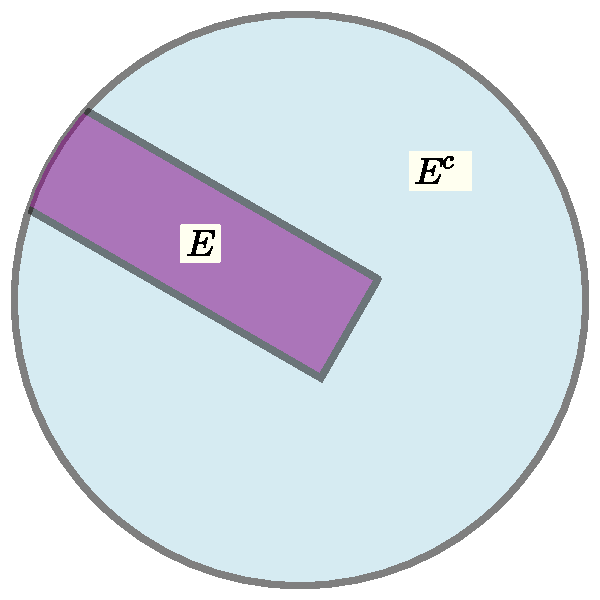
\includegraphics{039-2.pdf}}
\end{tabular}
\end{center}

\end{frame}

%%%%%%%%%%%%%%%%%%%%%%%%%%%%%%%%%%%%%%%%%%%%%%%%%%%%%%%%%%%%
\begin{frame}
\frametitle{Disjoint events}

Two events are {\bf disjoint} if they contain no points in common.
These two events are disjoint:

\begin{center}
\begin{tabular}{ll}
E1:& A person's birthday is on the 31st day of the month\\
E2:& A person's birthday is in June
\end{tabular}
\end{center}

\end{frame}

%%%%%%%%%%%%%%%%%%%%%%%%%%%%%%%%%%%%%%%%%%%%%%%%%%%%%%%%%%%%
\begin{frame}
\frametitle{Disjoint events}

But these events are not disjoint:

\begin{center}
\begin{tabular}{ll}
E1:& A person's birthday is on a Tuesday\\
E2:& A person's birthday is in June
\end{tabular}
\end{center}

\end{frame}

%%%%%%%%%%%%%%%%%%%%%%%%%%%%%%%%%%%%%%%%%%%%%%%%%%%%%%%%%%%%
\begin{frame}
\frametitle{Disjoint events}

Events $E1$ and $E2$ are disjoint on the left, but not on the
right. The large gray circle represents the full sample space.

\begin{center}
\begin{tabular}{cc}
\scalebox{0.4}{\includegraphics{040-1.pdf}}&
\scalebox{0.4}{\includegraphics{040-2.pdf}}
\end{tabular}
\end{center}

\end{frame}


%%%%%%%%%%%%%%%%%%%%%%%%%%%%%%%%%%%%%%%%%%%%%%%%%%%%%%%%%%%%
\begin{frame}
\frametitle{Disjoint events}

If events $E1$ and $E2$ are disjoint, then the probability of at least
one of them happening is the sum of their probabilities:

$$
P(E1\;{\rm or}\;E2) = P(E1) + P(E2).
$$
\end{frame}

%%%%%%%%%%%%%%%%%%%%%%%%%%%%%%%%%%%%%%%%%%%%%%%%%%%%%%%%%%%%
\begin{frame}
\frametitle{Example: Disjoint events}
Roll a fair die, and consider these events:

\begin{center}
\begin{tabular}{ll}
E1:& The result is even\\
E2:& The result is a 3 or a 5
\end{tabular}
\end{center}

The event ``$E1$ or $E2$'' is the event that I get a 2, 3, 4, 5, or 6.
This event has probability $5/6$.  Since $P(E1) = 1/2$ and $P(E2) =
1/3$, we can check that $P(E1\;{\rm or}\;E2) = 5/6 = 1/2 + 1/3 = P(E1)
+ P(E2)$.

\end{frame}

%%%%%%%%%%%%%%%%%%%%%%%%%%%%%%%%%%%%%%%%%%%%%%%%%%%%%%%%%%%%
\begin{frame}
\frametitle{Disjoint events}

Now consider these events:

\begin{center}
\begin{tabular}{ll}
E1:& The result is even\\
E2:& The result is less than or equal to 3
\end{tabular}
\end{center}

These events are not disjoint, since 2 is in both events.

The event ``$E1$ or $E2$'' is the event that I get a 1, 2, 3, 4, or 6.
This event has probability $5/6$.  But $P(E1) = 1/2$ and $P(E2) = 1/2$
so $P(E1)+P(E2) \ne P(E1\;{\rm or}\;E2)$.

\end{frame}

%%%%%%%%%%%%%%%%%%%%%%%%%%%%%%%%%%%%%%%%%%%%%%%%%%%%%%%%%%%%
\begin{frame}
\frametitle{Exercises}

Suppose we are considering a population of students that is 52\%
female, and for which 40\% of the students have visited a doctor in
the last year.

\begin{itemize}

\item If these events are independent, what is the probability that a
  randomly sampled student is a male who has not seen a doctor in the
  last year?

\item If these events are independent, what is the probability that a
  randomly sampled student is either a male who has not seen a doctor
  in the last year, or is a female who has not seen a doctor in the
  last year?

\item If there are 1000 students in our population, and gender is
  independent of whether a student visited a doctor in the past year,
  how many students are females who have not seen a doctor in the past
  year?

\end{itemize}

\end{frame}

%%%%%%%%%%%%%%%%%%%%%%%%%%%%%%%%%%%%%%%%%%%%%%%%%%%%%%%%%%%%
\begin{frame}
\frametitle{Answers}


\begin{itemize}

\item $P(Student=Male) = 0.48$, and $P(StudentNoSeenDoctorLastYear) = 0.6$ (both are complements of the events given in the exercise).  By
  independence, $P(Student=Male,And,StudentNoSeenDoctorLastYear) = 0.48*0.6 = 0.288$.

\item Simalalry $P(Student=Female,And,StudentNoSeenDoctorLastYear) = 0.52*0.6 =
  0.312$.  These events are disjoint, so the probability of one or the
  other occuring is 0.288+0.312 = 0.6.  It's not a coincidence that
  this is equal to 1-0.4, the probability of visiting a doctor
  regardless of gender.

\item The probability that a student is a female who has not seen a
  doctor in the last year is 0.312, so the number of such people is
  1000*0.312 = 312.

\end{itemize}

\end{frame}

%%%%%%%%%%%%%%%%%%%%%%%%%%%%%%%%%%%%%%%%%%%%%%%%%%%%%%%%%%%
%\begin{frame}{Probability, continued} 
%\begin{example}
%If we choose a real number $x$ from the interval $[0,5]$, what is the probability that $2\leq x \leq 4$?  In this case, $S=[0,5]$ and $A=[2,4]$.  It follows that $P(A)= 2/5$.
%\end{example}
%
%\begin{example}
%\begin{center}
%%\includegraphics[width=3cm]{circle.png}
%\end{center}
%If we choose a point from the square above, the probability that the point belongs to the shaded region equals  $\frac{(2r)^2-\pi r^2}{(2r)^2}= 1-\frac{\pi}{4}= 0.215$.
%\end{example}
%\end{frame}

%%%%%%%%%%%%%%%%%%%%%%%%%%%%%%%%%%%%%%%%%%%%%%%%%%%%%%%%%%
\begin{frame}{Axioms* of Probability}
\begin{itemize}
\item Probability is between 0 and 1. ie $P(E) \in [0,1]$
\item Outcome is always from the sample space.
\item Summation of probabilities of all possible outcomes is 1
\end{itemize}

* Axioms are statements considered to be true without any proof.
\end{frame}



%%%%%%%%%%%%%%%%%%%%%%%%%%%%%%%%%%%%%%%%%%%%%%%%%%%%%%%%%%
\begin{frame}{Properties of Probability}
Let $S$ be the sample space and $A,B$ be events.  Then
\begin{itemize}
\item $P(S)=1, P(\emptyset)=0$. 
\item If $A\subseteq B$, then $P(A)\leq P(B)$.  In particular, $0\leq P(A)\leq 1$. 
\item $P(A\cup B)=P(A)+P(B)-P(A\cap B)$.  In particular, if $A$ and $B$ are disjoint, then $P(A
\cup B)=P(A)+P(B)$. 
\item $P(A^c)=1-P(A)$.
\end{itemize}
\end{frame}


%%%%%%%%%%%%%%%%%%%%%%%%%%%%%%%%%%%%%%%%%%%%%%%%%%%%%%%%%%
\begin{frame}
\frametitle{Visualizing Probability}
\begin{itemize}
\item  Let rectangular region being of entire sample space. Area is ``1''.
\item Points are outcomes
\item Events are collection of outcomes, so sub-regions.
\item Probability is shown as area of the sub-region.
\end{itemize}

\begin{center}
\includegraphics[width=0.5\linewidth,keepaspectratio]{math2}
\end{center}

\tiny{(Ref: Math for Machine Learning - AWS Brent Werness)}
\end{frame}

%%%%%%%%%%%%%%%%%%%%%%%%%%%%%%%%%%%%%%%%%%%%%%%%%%%%%%%%%%
\begin{frame}
\frametitle{Visualizing Probability}
\begin{itemize}
\item  Union of Events is sum of probability when they are Exclusive.
\item If they are not, meaning there is some intersection between events, then total probability is sum of both minus the intersection (as it got included twice)
\item For 3 events summation, add all 3, minus 3 double overlaps, plus add single triple overlap.
\end{itemize}

\begin{center}
\includegraphics[width=0.5\linewidth,keepaspectratio]{math3}
\end{center}

\tiny{(Ref: Math for Machine Learning - AWS Brent Werness)}
\end{frame}

